% Chapter 2

\chapter{CMS Detector} % 

\label{Chapter 2} % For referencing the chapter elsewhere, use \ref{Chapter1} 

\lhead{Chapter 2. \emph{CMS Detector}} % This is for the header on each page - perhaps a shortened title

%----------------------------------------------------------------------------------------
The Compact Muon Solenoid (CMS \cite{CMSTDR}) is one of two general purpose detectors at the LHC which have performed exceptionally well during run 1. It is described in detail in \cite{CMS}. 

\begin{figure}
\centering
    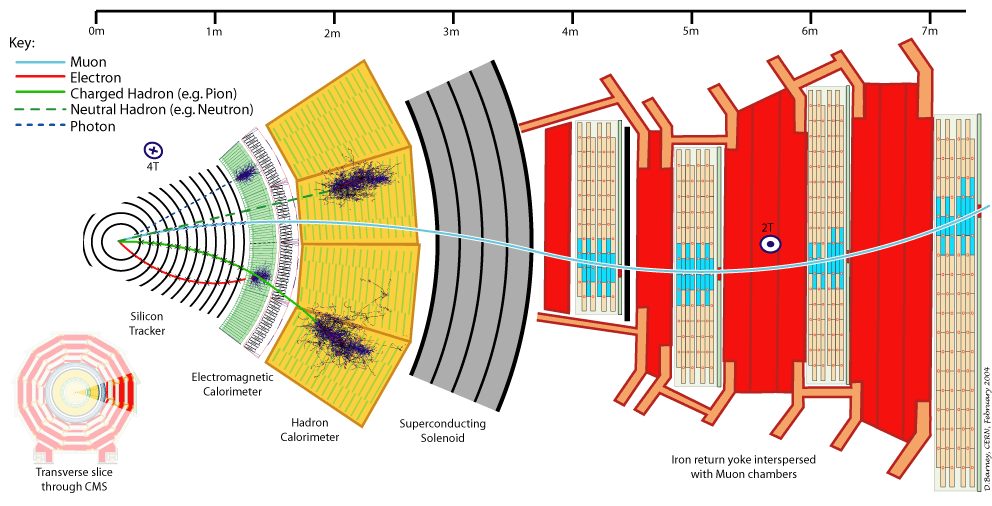
\includegraphics[width=0.9\textwidth]{./Figures/CMS_Slice.jpg}
  \caption{Cross Section of CMS showing the paths of various particle types through different segments of the detector \cite{cmsslice}}
  \label{CMS_SLICE}
\end{figure}

A cross section of CMS is shown in figure \ref{CMS_SLICE}. The coordinate system used by CMS takes the origin at the collision point. The z-axis points along the beam direction and defines the azimuthal angle, $\phi$. Instead of the polar angle, $\theta$, the psuedorapidity, $\eta=-ln(tan(\theta/2))$, is used as $\Delta \eta$ between two particles is approximately relativistically invariant. The eta coverage of CMS is $|\eta|<5$. Transverse energies and momenta ($E_T $ and $p_T$)  are defined perpendicular to the beam \cite{cmsiop}. The different detector components shown in figure \ref{CMS_SLICE} will now be described in detail. Resolutions are quoted for measuring the relevant property for a 100 GeV particle/jet \cite{SACharacteristics}.
\begin{description}
\item[Silicon Tracker]The job of the tracker is to measure the momentum of charged particles from their path through a magnetic field \cite{siliconTDR}. The CMS tracker achieves $10\mu m$ accuracy with coverage for $|\eta|<2.5$ and has a resolution of 1\%.
\item[Electromagnetic Calorimeter (ECAL)] The ECAL measures the energy of incident photons and electrons. The ECAL barrel is made of 61,200 $PbWO_4$ crystals and provides coverage for $|\eta|<1.48$ \cite{ecal}. This is extended to $|\eta|<3$ by the endcap which adds another $10764$ crystals. The endcap has a pre-shower to distinguish between $\gamma$ and $\pi^0$. The ECAL has a resolution of 0.5\%.
 \item[Hadronic Calorimeter (HCAL)] The HCAL is made from alternating brass and scintilator layers with a coverage of $|\eta|<3.0$ \cite{hcal}. The coverage is extended to  $|\eta|<5.0$ by an iron/quartz forward calorimeter \cite{hfhcal}. The average resolution is 11\%. 
 \item[Muon Chambers]The muons are not stopped by any of the calorimeters and therefore require a separate detector with coverage $|\eta| < 2.4$. The muon chambers are interspersed with the magnet return yoke. The high magnetic field allows for accurate momentum measurement \cite{muons}. The resolution is 1\%.
\end{description}
As the data rate ($40Mhz$) is far too high for every event to be stored and as new physics will only be seen in a minority of events a trigger system for interesting events is necessary. This happens in two stages: the L1 
Calorimetric and Muon Trigger (Hardware) and the High Level Trigger (Software) \cite{HLT}. The L1 trigger must operate within $\mathcal{O}10ns$ and so  the calorimetric trigger only takes input from the ECAL and HCAL. This is described in more detail in chapter \ref{Chapter3}. The input from the L1 triggers is then combined in the Global Trigger (GT) which decides whether to keep the event. The $\mathcal{O}100kHz$ events which pass L1 selection are processed in the HLT which utilises the calorimeter information along with tracking and the muon system to further reduce the rate to $\mathcal{O}1kHz$.
